%%%%%%%%%%%%%%%%%%%%%%%%%%%%%%%%%%%%%%%%%%%%%%%%%%%%%%%%%%%%%%%%%%%%%%%%%%%%%%%
\documentclass[hyperref={pdfpagelabels=false},compress,table]{beamer} % 在Mac下无法编译
% \documentclass[compress,table]{beamer} % 在Mac下使用
% package for font
\usepackage{fontspec}
\defaultfontfeatures{Mapping=tex-text}  %%如果没有它,会有一些 tex 特殊字符无法正常使用,比如连字符。
\usepackage{xunicode,xltxtra}
\usepackage[BoldFont,SlantFont,CJKnumber,CJKchecksingle]{xeCJK}  % \CJKnumber{12345}: 一万二千三百四十五
\usepackage{CJKfntef}  %%实现对汉字加点、下划线等。
\usepackage{pifont}  % \ding{}
% package for math
\usepackage{amsfonts}

% package for graphics
\usepackage[americaninductors,europeanresistors]{circuitikz}
\usepackage{tikz}
\usetikzlibrary{plotmarks}  % placements=positioning
\usepackage{graphicx}  % \includegraphics[]{}
\usepackage{subfigure}  %%图形或表格并排排列
% package for table
\usepackage{colortbl,dcolumn}  %% 彩色表格
\usepackage{multirow}
\usepackage{multicol}
\usepackage{booktabs}
% package for code
\usepackage{fancyvrb}
\usepackage{listings}

% \usepackage{animate}
% \usepackage{movie15}

%%%%%
% setting for beamer
\usetheme{default} % Madrid(常用), Copenhagen, AnnArbor, boxes(白色), Frankfurt,Berkeley
\useoutertheme[subsection=true]{miniframes} % 使用Berkeley时注释本行
\usecolortheme{sidebartab}
\usefonttheme{serif}  %%英文使用衬线字体
% \setbeamertemplate{background canvas}[vertical
% shading][bottom=white,top=structure.fg!7] %%背景色,上25%的蓝,过渡到下白。
\setbeamertemplate{theorems}[numbered]
\setbeamertemplate{navigation symbols}{}  %% 去掉页面下方默认的导航条
\setbeamercovered{transparent}  %设置 beamer 覆盖效果

% 设置标题title背景色
% \setbeamercolor{title}{fg=black, bg=lightgray!60!white}
\setbeamercolor{title}{fg=white, bg=black!70!white}

% 设置每页小LOGO
\pgfdeclareimage[width=1cm]{ouc}{figures/static/ouc.pdf}
\logo{\pgfuseimage{ouc}{\vspace{-20pt}}}

% setting for font
%%\setCJKmainfont{Adobe Kaiti Std}
\setCJKmainfont{SimSun} 
%% \setCJKmainfont{FangSong_GB2312} 
%% \setmainfont{Apple Garamond}  %%苹果字体没有SmallCaps
\setCJKmainfont{SimSun} 
%FUNNY%\setCJKmainfont{DFPShaoNvW5-GB}  %%华康少女文字W5(P)
%FUNNY%\setCJKmainfont{FZJingLeiS-R-GB}  %%方正静蕾体
%FUNNY%\setmainfont{Purisa}
%\setsansfont[Mapping=tex-text]{Adobe Song Std}
     %如果装了Adobe Acrobat,可在font.conf中配置Adobe字体的路径以使用其中文字体。
     %也可直接使用系统中的中文字体如SimSun、SimHei、微软雅黑等。
     %原来beamer用的字体是sans family;注意Mapping的大小写,不能写错。
     %设置字体时也可以直接用字体名,以下三种方式等同:
     %\setromanfont[BoldFont={黑体}]{宋体}
     %\setromanfont[BoldFont={SimHei}]{SimSun}
     %\setromanfont[BoldFont={"[simhei.ttf]"}]{"[simsun.ttc]"}
% setting for graphics
\graphicspath{{figures/}}  %%图片路径
\renewcommand\figurename{图}

% setting for pdf
\hypersetup{% pdfpagemode=FullScreen,%
            pdfauthor={Xiaodong Wang},%
            pdftitle={Title},%
            CJKbookmarks=true,%
            bookmarksnumbered=true,%
            bookmarksopen=false,%
            plainpages=false,%
            colorlinks=true,%
            citecolor=green,%
            filecolor=magenta,%
            linkcolor=blue,%red(default)
            urlcolor=cyan}

% setting for fontspec
\XeTeXlinebreaklocale "zh"  %%表示用中文的断行
\XeTeXlinebreakskip = 0pt plus 1pt minus 0.1pt  %%多一点调整的空间
%%%%%

% font setting by xeCJK
\setCJKfamilyfont{NSimSun}{NSimSun}
\newcommand{\song}{\CJKfamily{NSimSun}}
%%%\setCJKfamilyfont{AdobeSongStd}{Adobe Song Std}
%%%\newcommand{\AdobeSong}{\CJKfamily{AdobeSongStd}}
\setCJKfamilyfont{FangSong}{FangSong_GB2312}
\newcommand{\fang}{\CJKfamily{FangSong}}
%%%\setCJKfamilyfont{AdobeFangsongStd}{Adobe Fangsong Std}
%%%\newcommand{\AdobeFang}{\CJKfamily{AdobeFangsongStd}}
\setCJKfamilyfont{SimHei}{SimHei}
\newcommand{\hei}{\CJKfamily{SimHei}}
%%%\setCJKfamilyfont{AdobeHeitiStd}{Adobe Heiti Std}
%%%\newcommand{\AdobeHei}{\CJKfamily{AdobeHeitiStd}}
\setCJKfamilyfont{KaiTi}{KaiTi}
\newcommand{\kai}{\CJKfamily{KaiTi}}
%%%\setCJKfamilyfont{AdobeKaitiStd}{Adobe Kaiti Std}
\newcommand{\AdobeKai}{\CJKfamily{AdobeKaitiStd}}
\setCJKfamilyfont{LiSu}{LiSu}
\newcommand{\li}{\CJKfamily{LiSu}}
\setCJKfamilyfont{YouYuan}{YouYuan}
\newcommand{\you}{\CJKfamily{YouYuan}}
\setCJKfamilyfont{FZJingLei}{FZJingLeiS-R-GB}
\newcommand{\jinglei}{\CJKfamily{FZJingLei}}
\setCJKfamilyfont{MSYH}{Microsoft YaHei}
\newcommand{\msyh}{\CJKfamily{MSYH}}

% 自定义颜色
\def\Red{\color{red}}
\def\Green{\color{green}}
\def\Blue{\color{blue}}
\def\Mage{\color{magenta}}
\def\Cyan{\color{cyan}}
\def\Brown{\color{brown}}
\def\White{\color{white}}
\def\Black{\color{black}}

\lstnewenvironment{xmlCode}[1][]{% for Java
  \lstset{
    basicstyle=\tiny\ttfamily,%
    columns=flexible,%
    framexleftmargin=.7mm, %
    % frame=shadowbox,%
    % rulesepcolor=\color{cyan},%
     frame=single,%
    backgroundcolor=\color{white},%
    xleftmargin=4\fboxsep,%
    xrightmargin=4\fboxsep,%
    numbers=left,numberstyle=\tiny,%
    numberblanklines=false,numbersep=7pt,%
    language=xml, %
    }\lstset{#1}}{}

\lstnewenvironment{javaCode}[1][]{% for Java
  \lstset{
    basicstyle=\tiny\ttfamily,%
    columns=flexible,%
    framexleftmargin=.7mm, %
    frame=shadowbox,%
    rulesepcolor=\color{cyan},%
    % frame=single,%
    backgroundcolor=\color{white},%
    xleftmargin=4\fboxsep,%
    xrightmargin=4\fboxsep,%
    numbers=left,numberstyle=\tiny,%
    numberblanklines=false,numbersep=7pt,%
    language=Java, %
    }\lstset{#1}}{}

\lstnewenvironment{shCode}[1][]{% for Java
  \lstset{
    basicstyle=\scriptsize\ttfamily,%
    columns=flexible,%
    framexleftmargin=.7mm, %
    frame=shadowbox,%
    rulesepcolor=\color{brown},%
    % frame=single,%
    backgroundcolor=\color{white},%
    xleftmargin=4\fboxsep,%
    xrightmargin=4\fboxsep,%
    numbers=left,numberstyle=\tiny,%
    numberblanklines=false,numbersep=7pt,%
    language=sh, %
    }\lstset{#1}}{}

\newcommand\ask[1]{\vskip 4bp \tikz \node[rectangle,rounded corners,minimum size=6mm,
  fill=white,]{\Cyan \includegraphics[height=1.5cm]{question} \Large \msyh #1};}

\newcommand\wxd[1]{\vskip 4bp \tikz \node[rectangle,minimum size=6mm,
  fill=blue!60!white,]{\White \ding{118} \msyh #1};}

\newcommand\xyy[1]{\vskip 2bp \tikz \node[rectangle,minimum size=3mm,
  fill=black!80!white,]{\White \msyh\scriptsize #1};}

\newcommand\cxf[1]{\vskip 4bp \tikz \node[rectangle,rounded corners,minimum size=6mm,
  fill=orange!60!white,]{\White \ding{42} \msyh #1};}

\newcommand\samp[1]{\vskip 2bp \tikz \node[rectangle,minimum size=3mm,
  fill=white!100!white,]{\Mage\msyh \small CODE \ding{231} \Black #1};\vskip -8bp}

\newcommand\zhyfly[1]{\tikz \node[rectangle,rounded corners,minimum size=6mm,ball color=red!25!blue,text=white,]{#1};}

\setbeamerfont{frametitle}{series=\msyh} % 修改Beamer标题字体

\makeatletter
\newcommand{\Extend}[5]{\ext@arrow 0099{\arrowfill@#1#2#3}{#4}{#5}}
\makeatother


%%%%%%%%%%%%%%%%%%%%%%%%%%%%%%%%%%%%%%%%%%%%%%%%%%%%%%%%%%%%%%%%%%%%%%%%%%%%%%%
% \titlepage
\title[KevinW@OUC]{\hei {\huge Java EE企业应用系统设计}\\  
Java EE监听器编程}
\author[王晓东]{王晓东\\
  \href{mailto:wangxiaodong@ouc.edu.cn}{\footnotesize wangxiaodong@ouc.edu.cn}}
\institute[中国海洋大学]{\small 中国海洋大学}
\date{\today}
\titlegraphic{\vspace{-6em}
\includegraphics[height=6cm]{static/ouc.pdf}\vspace{-6em}}
%%%%%
\begin{document}
%% Delete this, if you do not want the table of contents to pop up at
%% the beginning of each subsection:
\AtBeginSection[]{                              % 在每个Section前都会加入的Frame
  \frame<handout:0>{
    \frametitle{\textbf{\hei 接下来…}}
    \tableofcontents[currentsection]
  }
}  %

\AtBeginSubsection[]                            % 在每个子段落之前
{
  \frame<handout:0>                             % handout:0 表示只在手稿中出现
  {
    \frametitle{\textit{\hei 接下来…}}\small
    \tableofcontents[current,currentsubsection] % 显示在目录中加亮的当前章节
  }
}
 \frame{\titlepage}

%%%%%%%%%%%%%%%%%%%%%%%%%%%%%%%%%%%%%%%%%%%%%%%%
\begin{frame}
\frametitle{参考书目}
\begin{enumerate}
\item 吕海东,张坤 编著,Java EE企业级应用开发实例教程,清华大学出版社,2010年8月
\end{enumerate}  
\end{frame}

 \begin{frame}
 \frametitle{本章学习目标}
 \begin{enumerate}
 \item 什么是监听器?
 \item 监听器的主要功能和类型
 \item 监听器的编程和配置
 \item 监听器的测试和应用实例
 \end{enumerate}  
 \end{frame}

\section*{大纲}
\frame{\frametitle{大纲} \tableofcontents}

\section{监听器概述}

\begin{frame}
\frametitle{概述} 

监听器,顾名思义就是能监测其他对象活动的对象,当监测的对象发生变化时,会自动运行监听器方法,完成特定的功能和任务。 

Java EE规范在Servlet 2.3中引入了监听器(Listener)规范。

监听器能够检测Web应用中如下的关键对象:

\begin{itemize}
\item ServletContext上下文
\item HttpSession会话
\item ServletRequest请求对象
\end{itemize}

\end{frame}

\begin{frame}[fragile] % [fragile]参数使得能够插入代码
\frametitle{监听器的基本功能} 
\begin{enumerate}\kai
\item {\hei 网站访问人数或次数计数器}\\
访问人数计数是所有综合门户网站的生命,是网站广告标价的基础。国内知名门户网站如搜狐,新浪等广告价格高,就在于其每日巨大的访问量所致。	
\item {\hei 网站登录用户人数和在线用户监测}\\
可以使用监听器完成Web应用已经登录人数和在线用户列表的登记处理。这是许多网上论坛,网上购物网站,Mail在线系统,即时通讯系统等必须具有的功能。
\item {\hei 日志记录}\\
对Web应用关键的事件进行记录,如Web服务器的启动和停止,用户的登录和注销等事件的登记,便于日后进行系统中追踪和维护。
\item {\hei 会话超时后的清理工作}\\
\end{enumerate}
\end{frame}

\section{Java EE监听器类型}

\begin{frame}[fragile] % [fragile]参数使得能够插入代码
\frametitle{Java EE监听器类型} 

\begin{enumerate}
\item ServletContext对象监听器
\item ServletContext对象属性监听器
\item HttpSession对象监听器
\item HttpSession对象属性监听器
\item HttpServletRequest对象监听器
\item HttpServletRequest属性监听器
\end{enumerate}
\end{frame}

\begin{frame}[fragile] % [fragile]参数使得能够插入代码
\frametitle{Java EE监听器类型} 

\begin{center}\small
\setlength{\extrarowheight}{1.5mm}
\rowcolors[]{1}{red!20}{red!10}
\begin{tabular}{l|c|l}
监听器接口 & 引入版本 & 监听器事件\\
ServletContextListener & 2.3 & ServletContextEvent\\
ServletContextAttributeListener & 2.3 & ServletContextAttributeEvent\\
HttpSessionListener & 2.3 & HttpSessionEvent\\
HttpSessionActivationListener & 2.3 & HttpSessionEvent\\
HttpSessionBindingListener & 2.3 & HttpSessionBindingEvent\\
ServletRequestListener & 2.4 & ServletRequestEvent\\
ServletRequestAttributeListener & 2.4 & ServletRequestAttributeEvent\\
\end{tabular}
\end{center}
\end{frame}

\section{ServletContext对象监听器}

\begin{frame}[fragile] % [fragile]参数使得能够插入代码
\frametitle{ServletContext对象监听器}

ServletContext对象监听器能监听该对象的创建和销毁二个关键的状态,并分别提供了不同的方法来实现对该对象创建和销毁的监听和处理。
\begin{enumerate}
\item JavaEE规范定义了ServletContext监听器接口,来规范监听器的编写,javax.serlvet.ServletContextListener。
\item 提供了ServletContext监听器事件类,javax.servlet.ServletContextEvent。
\item 定义了取得监听对象本身的方法。
\end{enumerate}
\end{frame}

\begin{frame}[fragile] % [fragile]参数使得能够插入代码
\frametitle{ServletContext对象监听器编程} 

\begin{enumerate}
\item 定义监听器类并实现javax.servlet.ServletContextListener接口。
\item 实现接口中定义的如下两个方法:
  \begin{itemize}
  \item public void contextInitialized(ServletContextEvent event) \\对象创建监听方法
  \item public void contextDestroyed(ServletContextEvent event) \\对象销毁监听方法
  \end{itemize}
\item ServletContextEvent类型对象中封装了ServeltContext对象,可以用于实现对Web应用信息的访问。
\end{enumerate}
\end{frame}

\begin{frame}[fragile] % [fragile]参数使得能够插入代码
\frametitle{ServletContext对象监听器示例} 

\begin{javaCode}
public class ApplicationStatusListener implements ServletContextListener {
  ...
  public void contextInitialized(ServletContextEvent event) {
    ServletContext application = event.getServletContext();
    application.setAttribute("userOnlineNumber", userOnlineNumber);
    WebVisitNumber = UserOnline.getVisitNumber();
    application.setAttribute("WebVisitNumber", WebVisitNumber);
  }
  public void contextDestroyed(ServletContextEvent event) {
    ServletContext application = event.getServletContext();
    WebVisitNumber = (Integer) application.getAttribute("WebVisitNumber");
    UserOnline.saveVisitNumber(userOnlineNumber);
  }
}  
\end{javaCode}

\begin{itemize}\kai
\item 监听器监测到ServletContext对象创建,自动执行contextInitialized方法,取得以前保存的网站访问次数,将历史访问次数存入ServletContext对象中。将来监测到用户访问网站时,自动进行计数器累加。
\item 监听器检测到ServletContext对象要销毁,Web容器自动执行contextDestroyed方法,完成从ServletContext对象中取得累计访问次数并写入数据库中。
\end{itemize}
\end{frame}

\begin{frame}[fragile] % [fragile]参数使得能够插入代码
\frametitle{ServletContext 对象监听器配置} 

在/WEB-INF/web.xml中进行配置。

\begin{xmlCode}
<!-- ServletContext对象创建和销毁监听器 -->
<listener>  
  <listener-class>org.javaee.ApplicationStatusListener</listener-class>
</listener>  
\end{xmlCode}

不需要映射地址,也无需初始化参数,只需要监听器的包和类名即可。
\end{frame}

\section{ServletContext对象属性监听器}

\begin{frame}[fragile] % [fragile]参数使得能够插入代码
\frametitle{ServletContext对象属性监听器}

\wxd{需要被监控的属性变化}

Servlet作为Web应用级共享容器,可以使用如下操作ServletContext属性的方法
进行共享数据的保存、读取和删除:

\begin{itemize}
\item public void setAttribute(String name, Object value);
\item public Object getAttribute(String name);
\item public void removeAttribute(String name);
\end{itemize}
\end{frame}

\begin{frame}[fragile] % [fragile]参数使得能够插入代码
\frametitle{ServletContext对象属性监听器}

为监控ServletContext对象属性的变化,Java EE Servlet API提供了监听器接
口javax.servlet.ServletContextAttributeListener 和事件类
javax.servlet.ServletContextAttributeEvent,接口方法包括:

\begin{itemize}
\item public void attributeAdded(ServletContextAttributeEvent event);
\item public void attributeRemoved(ServletContextAttributeEvent
  event);
\item public void attributeReplaced(ServletContextAttributeEvent event);
\end{itemize}
\end{frame}

\begin{frame}[fragile] % [fragile]参数使得能够插入代码
\frametitle{ServletContext对象属性监听器}
\wxd{ServletContext对象属性监听器事件}

javax.servlet.ServletContextAttributeEvent对象是ServletContextEvent的
子类,其主要方法包括:

\begin{itemize}
\item 继承了父类方法public ServletContext getServletContext()取得
ServletContext对象的实例;
\item public String getName() 取得发生变化的属性的名称;
\item public Object getValue() 取得发生变化的属性的值。
\end{itemize}
\end{frame}

\begin{frame}[fragile] % [fragile]参数使得能够插入代码
\frametitle{ServletContext对象属性监听器示例}

\xyy{代码}

\begin{javaCode}
public class ApplicationAttributeListener implements
ServletContextAttributeListener {
  private String name = null;
  private String value = null;
  
  public void attributeAdded(ServletContextAttributeEvent event) {
    name = event.getName();
    value = (String) evnet.getValue();
    System.out.println("New Attribute added: " + "name" + "=" + "value");
  }

  // Other Methods.

}
\end{javaCode}
\xyy{配置}
\begin{xmlCode}
<!-- ServletContext对象创建和销毁监听器 -->
<listener>
  <listener-class>org.javaee.ApplicationAttributeListener</listener-class>
</listener> 
\end{xmlCode}
\end{frame}

%%%%%%%%%%%%%%%%%%%%%%%%%%
\begin{frame}[fragile] % [fragile]参数使得能够插入代码
\frametitle{} 

\end{frame}
%%%%%%%%%%%%%%%%%%%%%%%%%%
%% \begin{figure}
%% \centering
%% 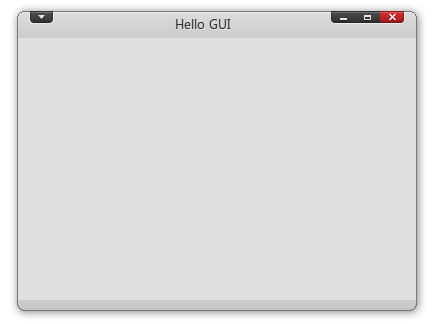
\includegraphics[width=0.6\textwidth]{fig01.png}
%% \end{figure}
% TKS %%%%%%%%%%%%%%%%%%%%%%%%%%%%%%%%%%%%%%%%%%%%%%
\begin{frame}
\centering
{\Huge \textcolor{blue}{THE END}} \\
\vspace{5mm}
{\Large wangxiaodong@ouc.edu.cn} \\
\end{frame}
%%%%%%%%%%%%%%%%%%%%%%%%%%%%%%%%%%%%%%%%%%%%%%%%%%
\end{document}
